\chapter{\posl{} Class diagrams}
\label{app:sgp}
\textit{In this chapter class diagrams of \posl{} are presented.}
\vfill
\newpage


\noindent\rule[2pt]{\textwidth}{0.8pt}

\clearpage

%\begin{figure}
%	\centering
%	\subfloat[][Data \opch]{
%		\label{subfig:doch}
%		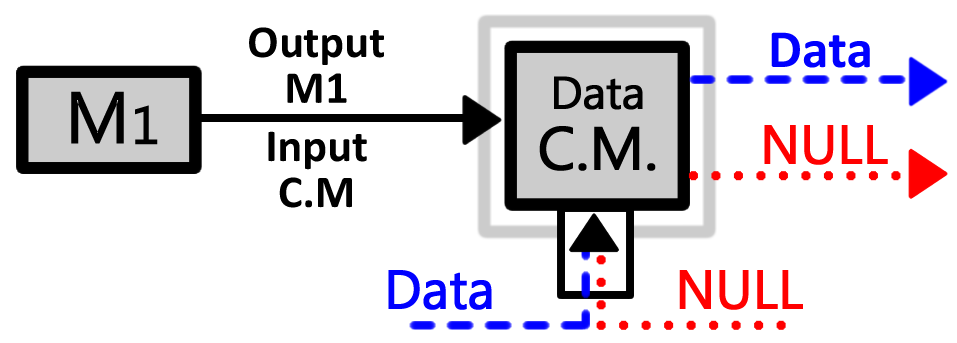
\includegraphics[width=0.4\linewidth]{D_OCh.png}
%	}
%	\hspace{0.05\textwidth}%
%	\subfloat[][Object \opch]{%
%		\label{subfig:ooch}
%		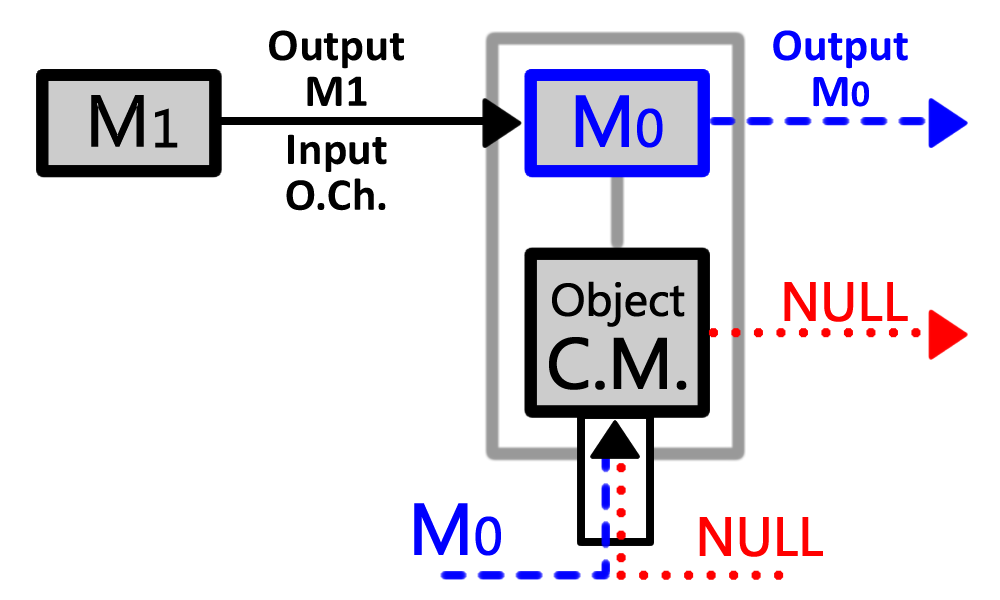
\includegraphics[width=0.4\linewidth]{O_OCh.png}
%	}
%	\caption[]{Communication module}
%	\label{fig:och}
%\end{figure}

\begin{figure}
	\centering
	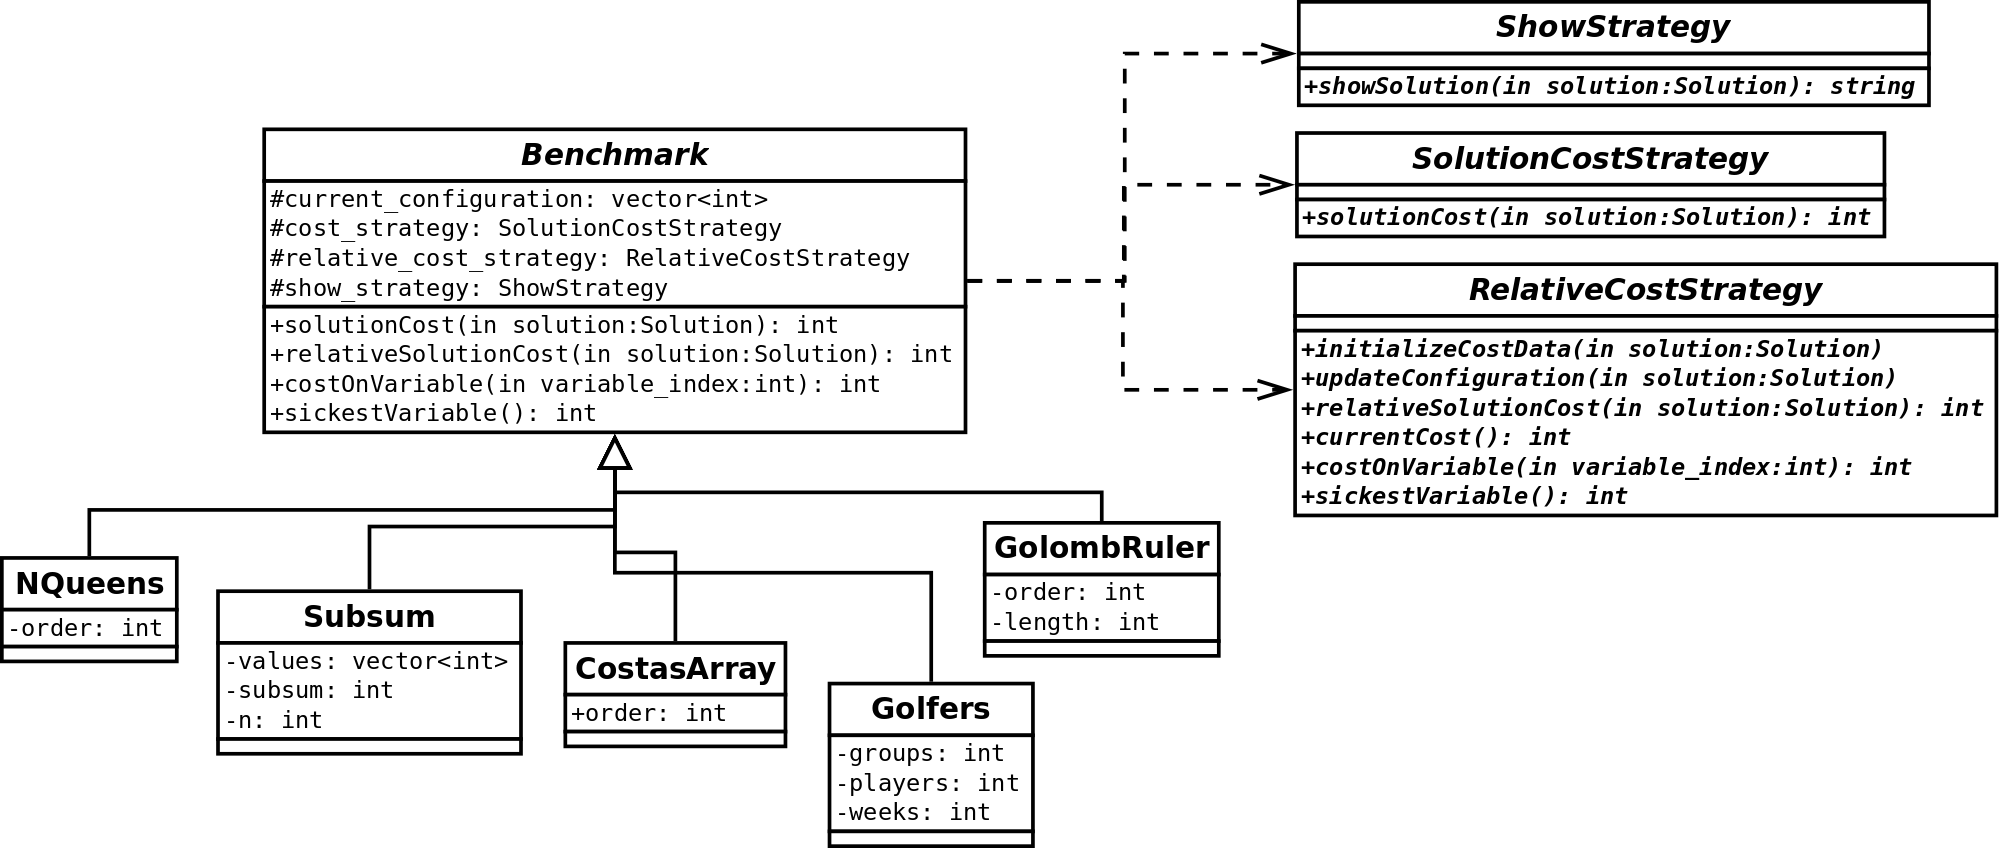
\includegraphics[width=\linewidth]{diabench.png}
	\caption[]{Benchmark class diagram}\label{diag:bench}
\end{figure}

\begin{figure}
	\centering
	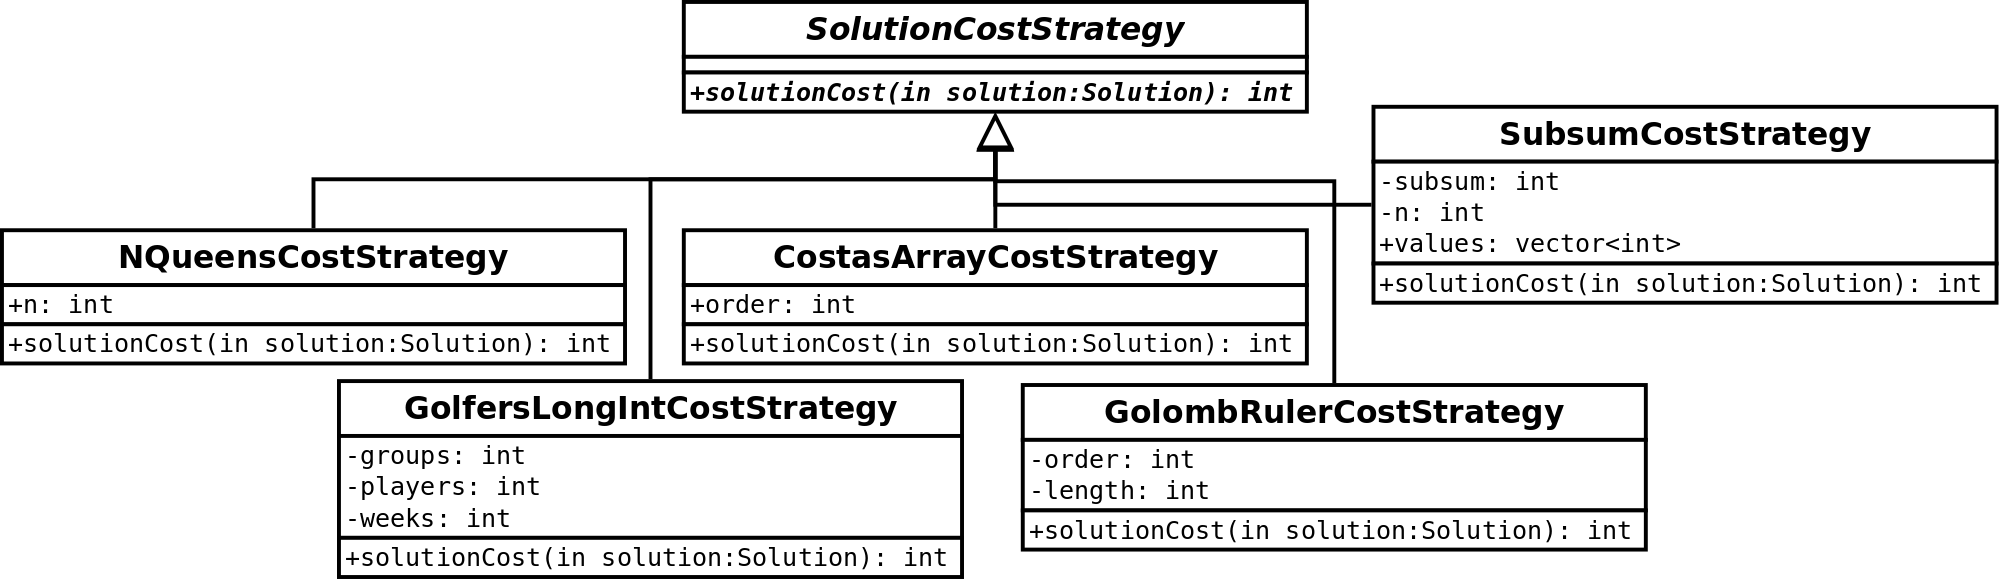
\includegraphics[width=\linewidth]{diacoststr.png}
	\caption[]{Cost strategy class diagram}\label{diag:coststr}
\end{figure}

\begin{figure}
	\centering
	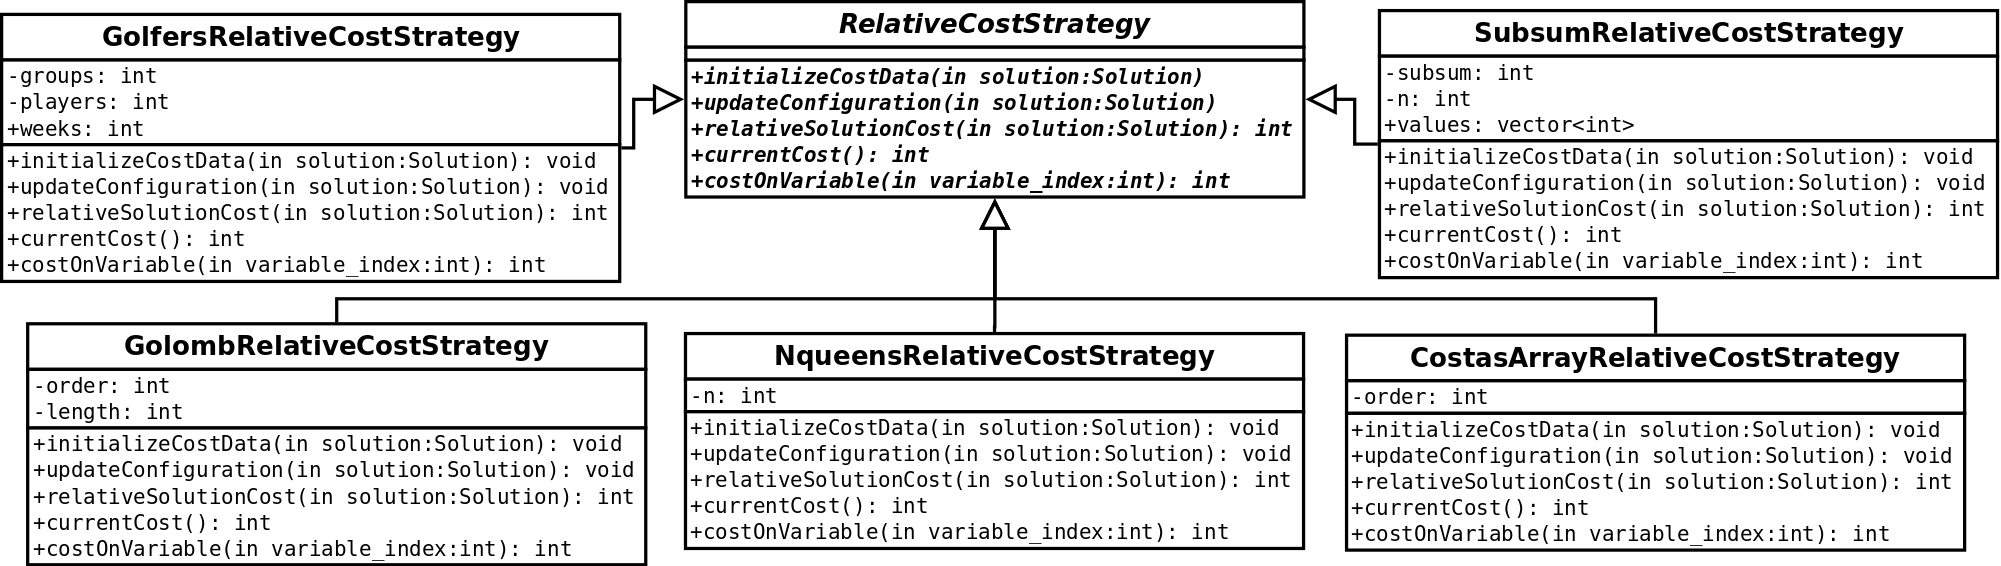
\includegraphics[width=\linewidth]{diarelacoststr.png}
	\caption[]{Relative cost strategy class diagram}\label{diag:relacoststr}
\end{figure}

\begin{figure}
	\centering
	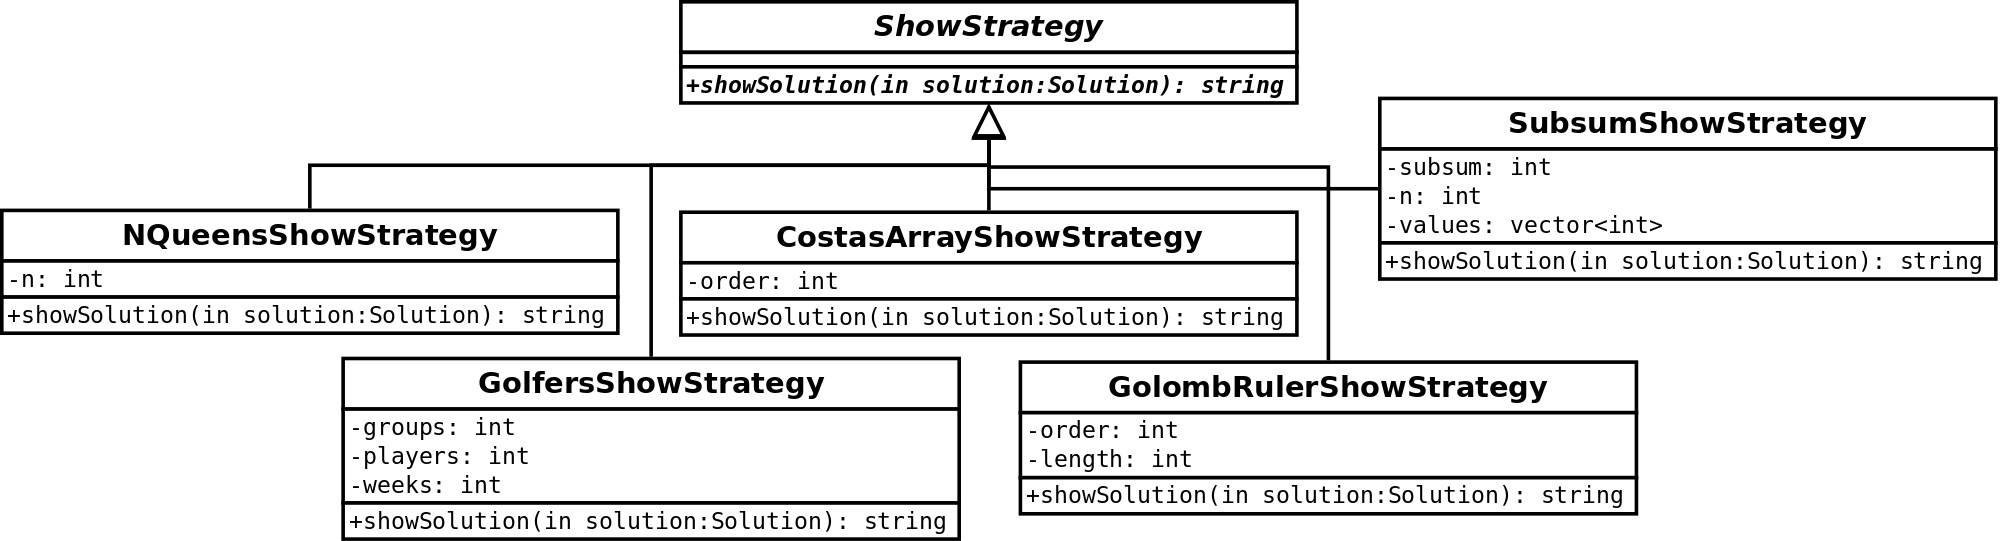
\includegraphics[width=\linewidth]{diashowstr.png}
	\caption[]{Show solution strategy class diagram}\label{diag:showstr}
\end{figure}

\begin{figure}
	\centering
	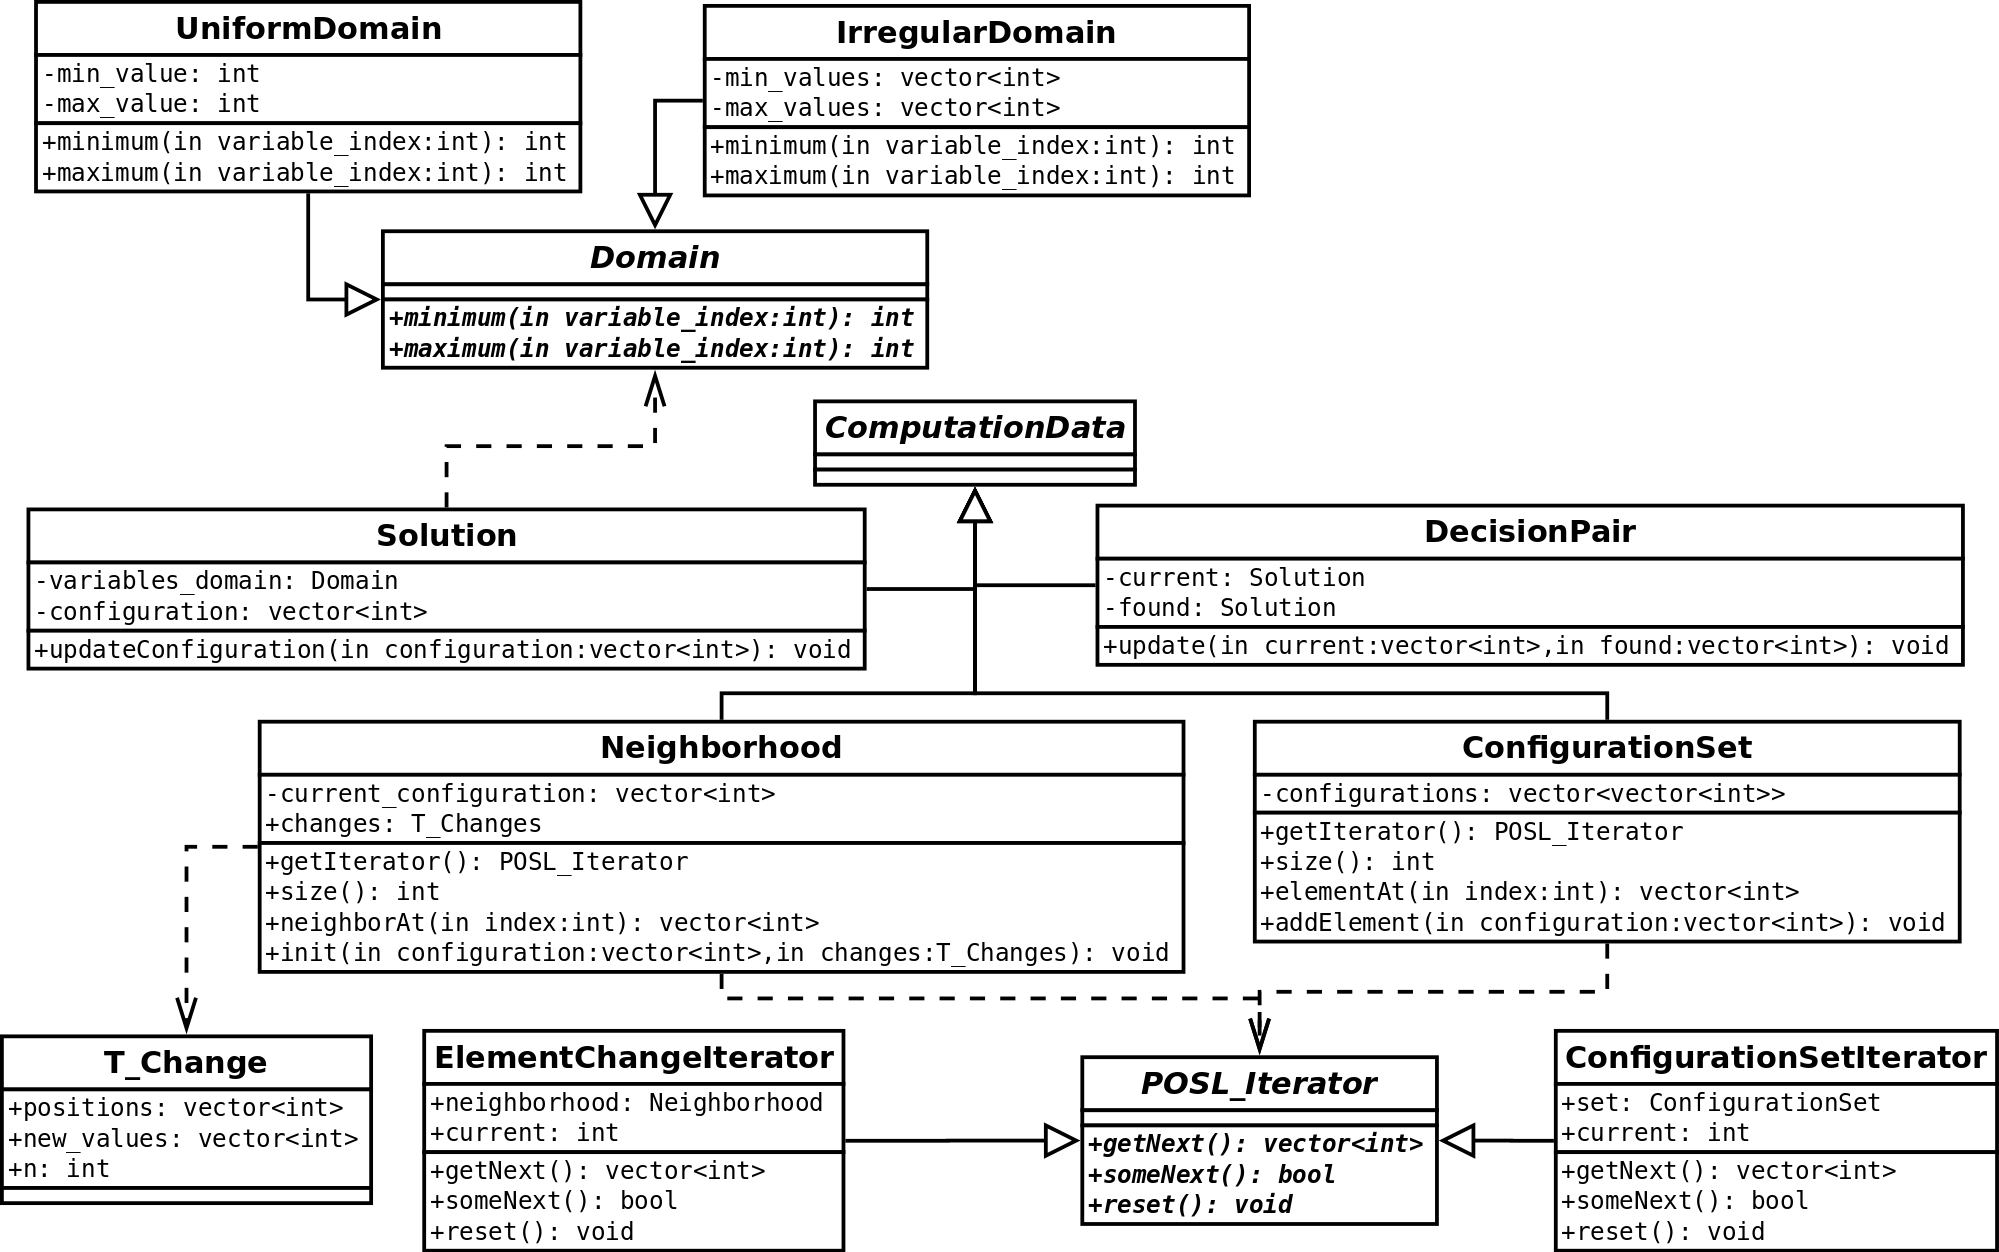
\includegraphics[width=\linewidth]{diadata.png}
	\caption[]{\posl{} data class diagram}\label{diag:data}
\end{figure}

\begin{figure}
	\centering
	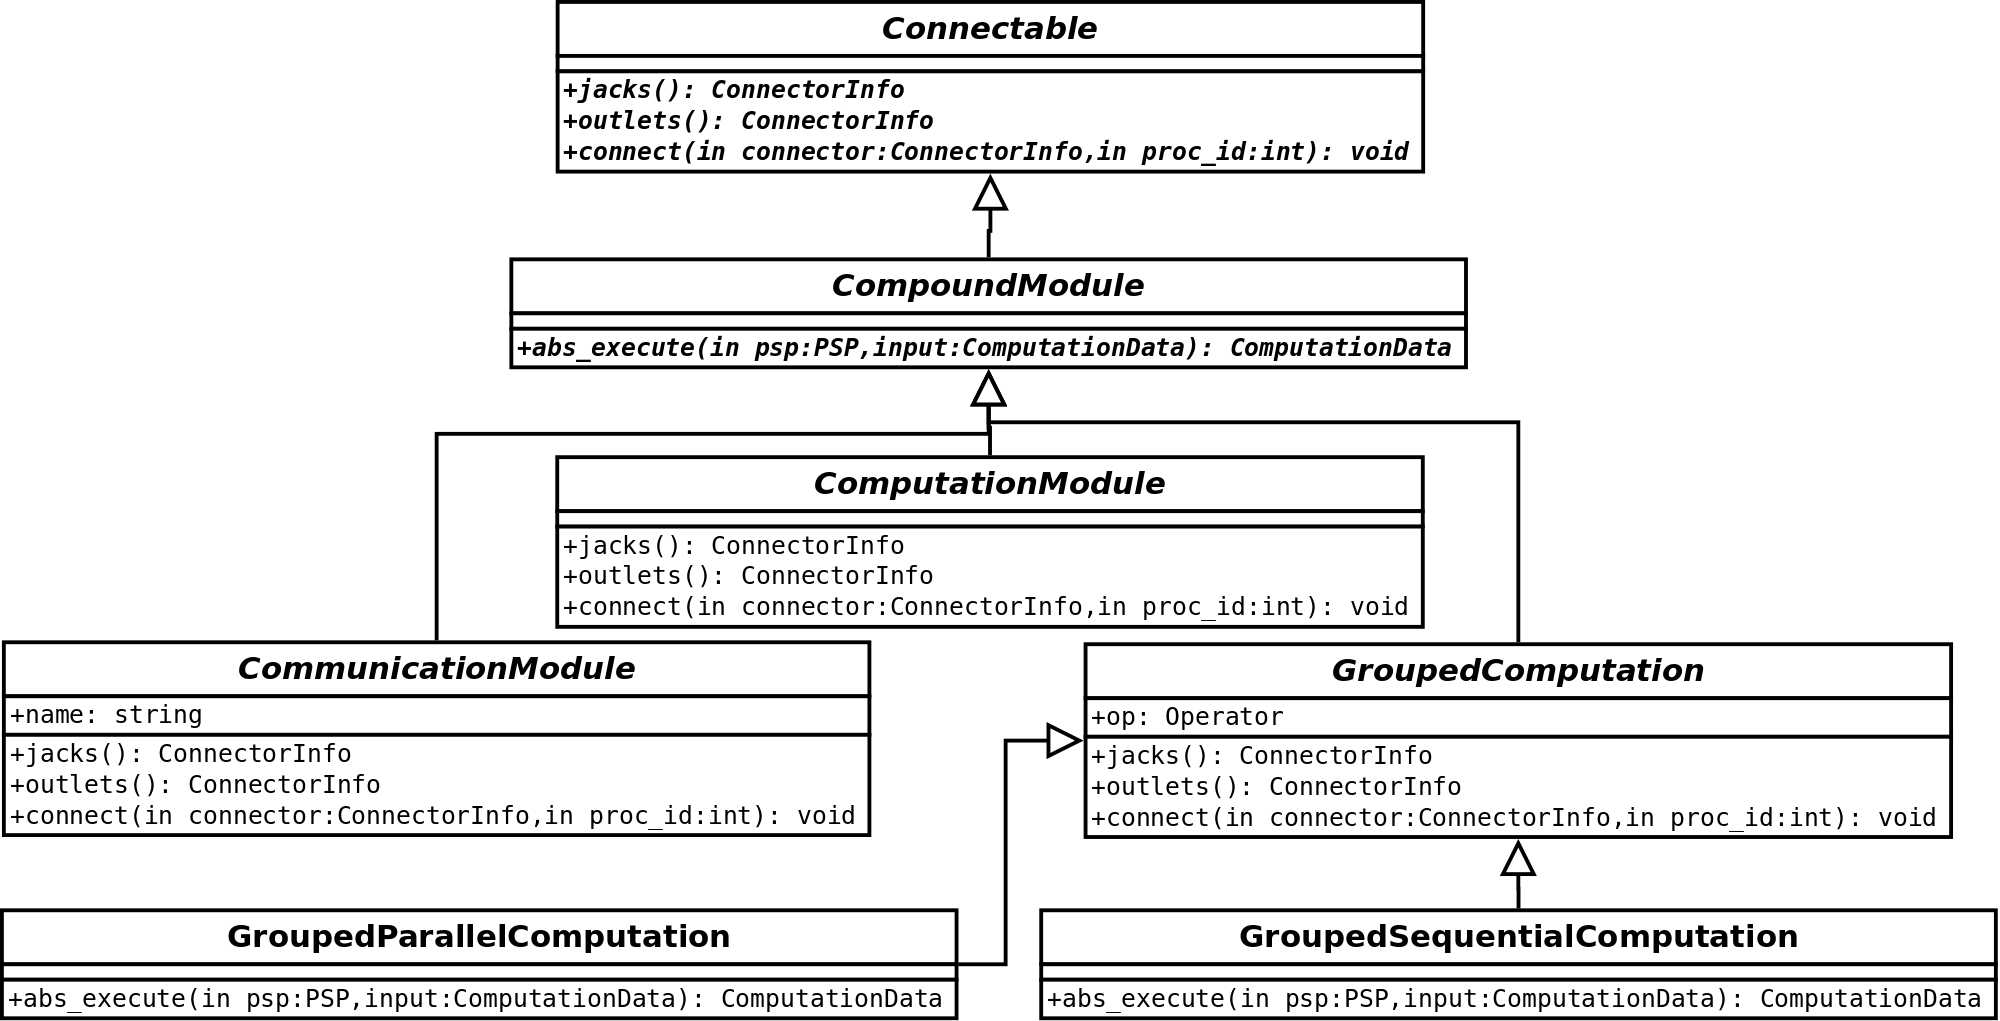
\includegraphics[width=\linewidth]{diacm.png}
	\caption[]{Compound modules class diagram}\label{diag:cm}
\end{figure}

\begin{figure}
	\centering
	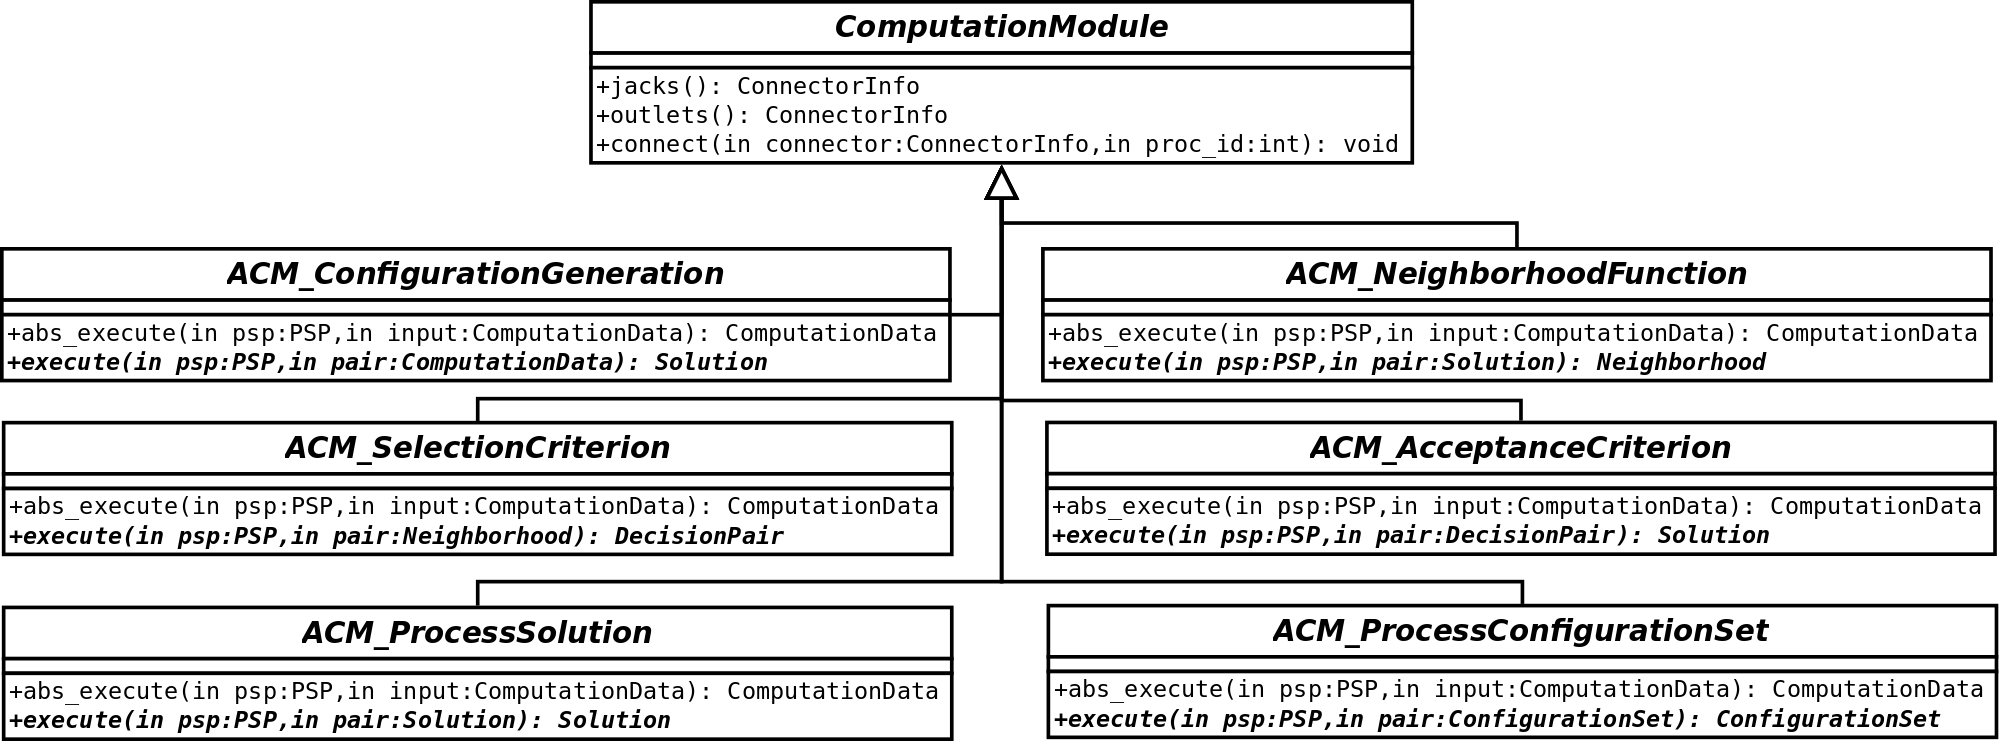
\includegraphics[width=\linewidth]{diaom.png}
	\caption[]{Abstract computation modules class diagram}\label{diag:om}
\end{figure}

\begin{figure}
	\centering
	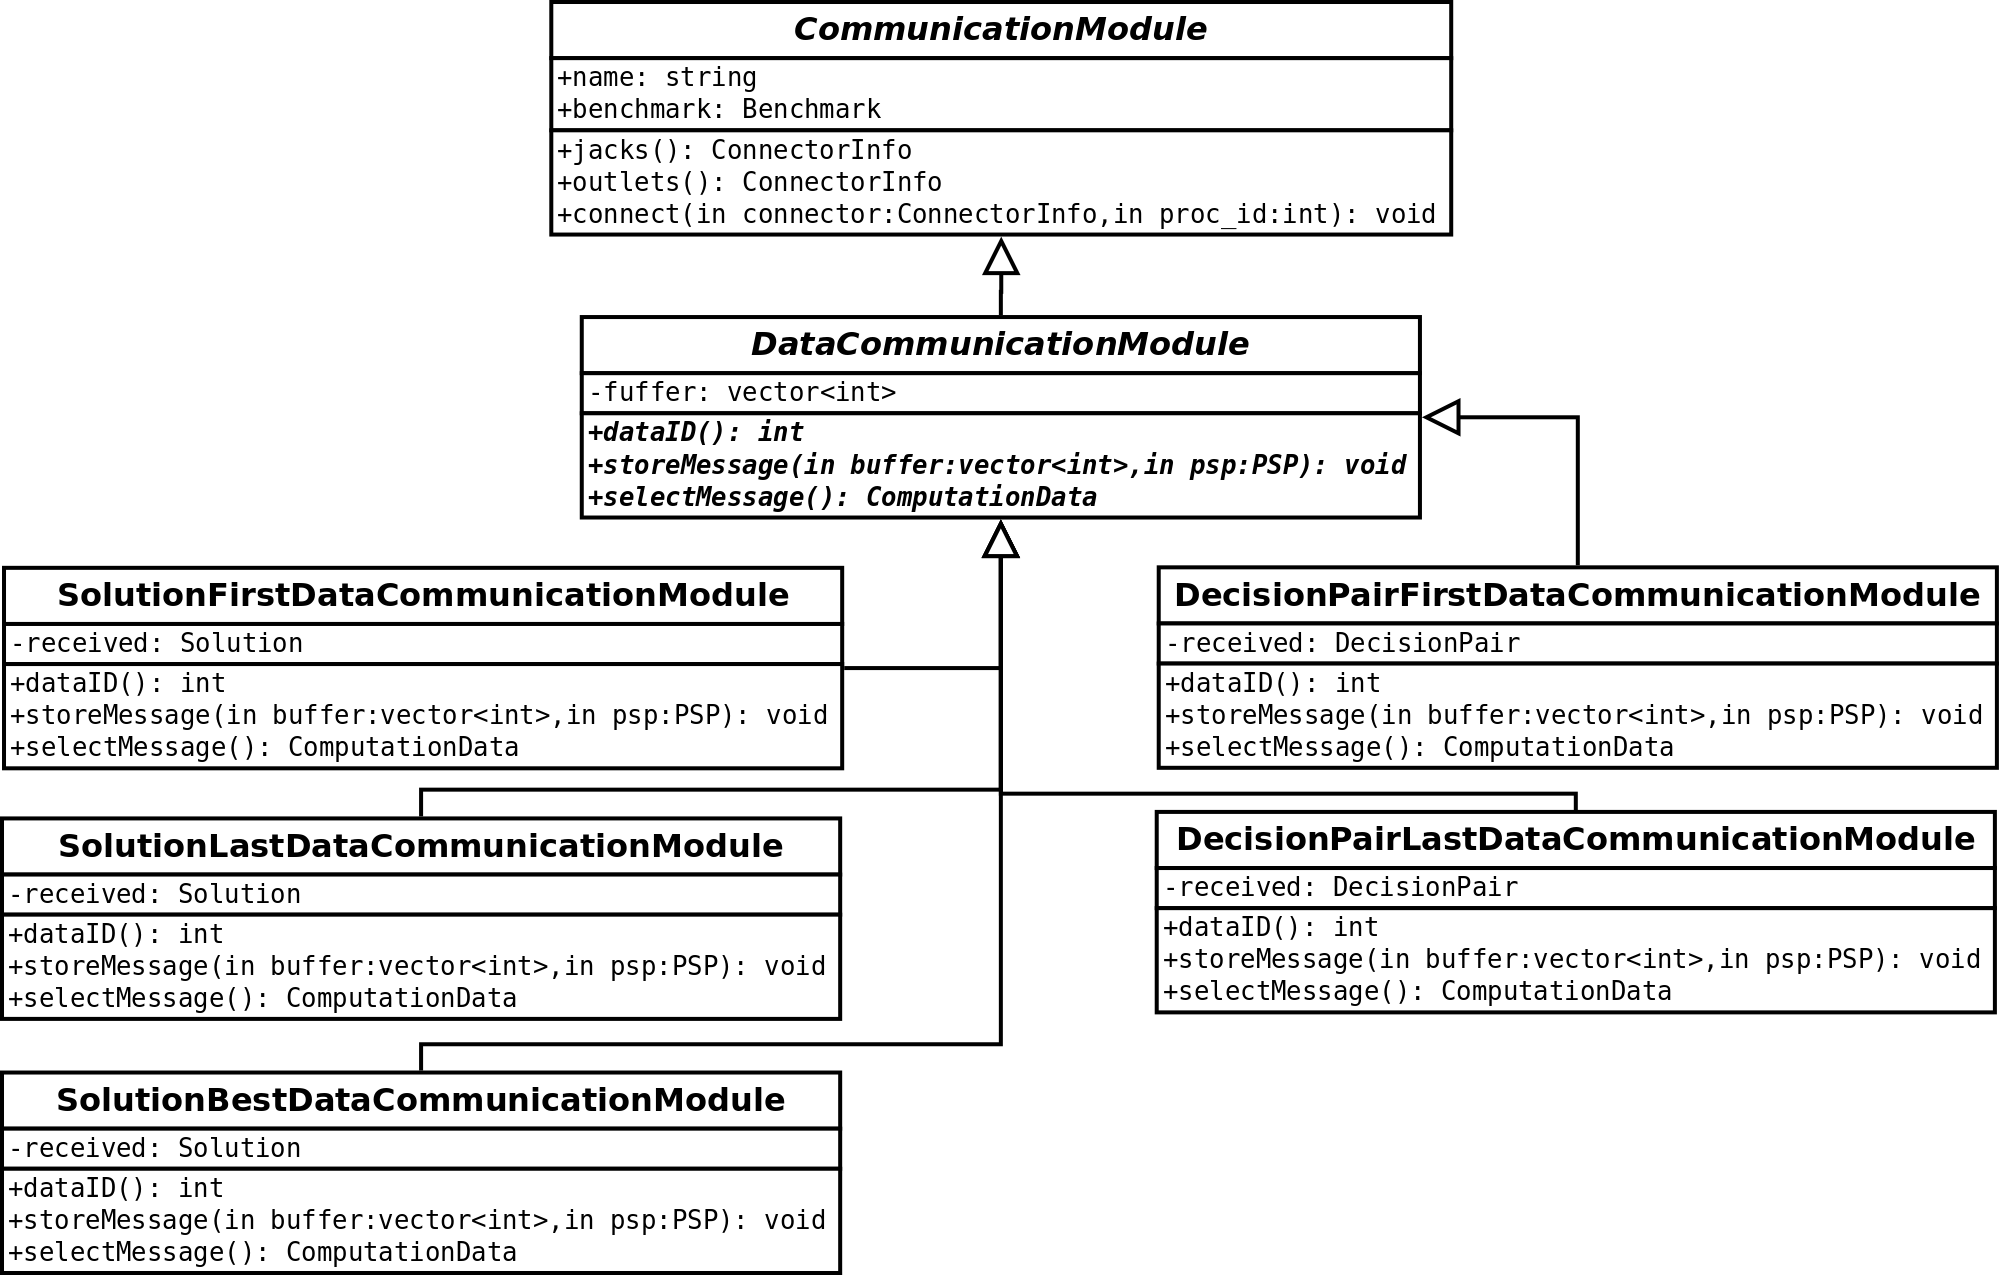
\includegraphics[width=\linewidth]{diaoch.png}
	\caption[]{Communication modules class diagram}\label{diag:opch}
\end{figure}